% ##################################################################################################################
\section{Tel Aviv}
\label{sec:telaviv}
\hfill \textbf{Author:} Christoph Dobler

% ##################################################################################################################
The initial Tel Aviv \gls{matsim} scenario \citep[][]{BekhorEtAl_TRB_2011} was recently extended by adding destination choice to the \gls{matsim} iterations \citep[][]{DoblerEtAl_TechRep_IVT_2014}.

The modeled area was divided into 1\,219\,\gls{taz} (Figure~\ref{fig:TAZ}). The geometry was provided as \gls{esri} shape file \citep{ESRI-ShapeFile_manual_1998}. The zonal attributes contained information related to the population living in the zone as well as the types of activities that can be performed.

The population was created based on the outcomes of the population generator from the Tel Aviv activity-based model containing socio-demographic attributes and daily schedules with up to six activities. The keep the computational effort manageable a 10\,\% population sample was simulated. Additional data has been provided for external trips. For each of the three types (car, truck, commercial), \gls{od} matrices for three different time periods (AM, OP, PM) were available.

Input data for the network was taken from the \gls{emme2} model \citep[see][]{EMME_Webpage_2011} which is also used by the Assignment Unit of the existing Tel Aviv Model. Details about the conversion process can be found in \citet{GaoWEtAl_TRR_2010}. Turning restrictions were considered by adapting the network structure, resulting in a network containing 9\,474\,nodes and 18\,570\,links (Figure~\ref{fig:network}). Capacities of some major roads were corrected manually because they were obviously too low (e.g.,\,noticeably lower than traffic counts indicated).

The Tel Aviv scenario contains road pricing of two arterial highways. Count data for validation was available for 3\,arterial roads.
%
\createfigure%
{Tel Aviv scenario}%
{Tel Aviv scenario}%
{\label{fig:telavivscenario}}%
{%
  \createsubfigure%
  {\protect\gls{taz}}%
  {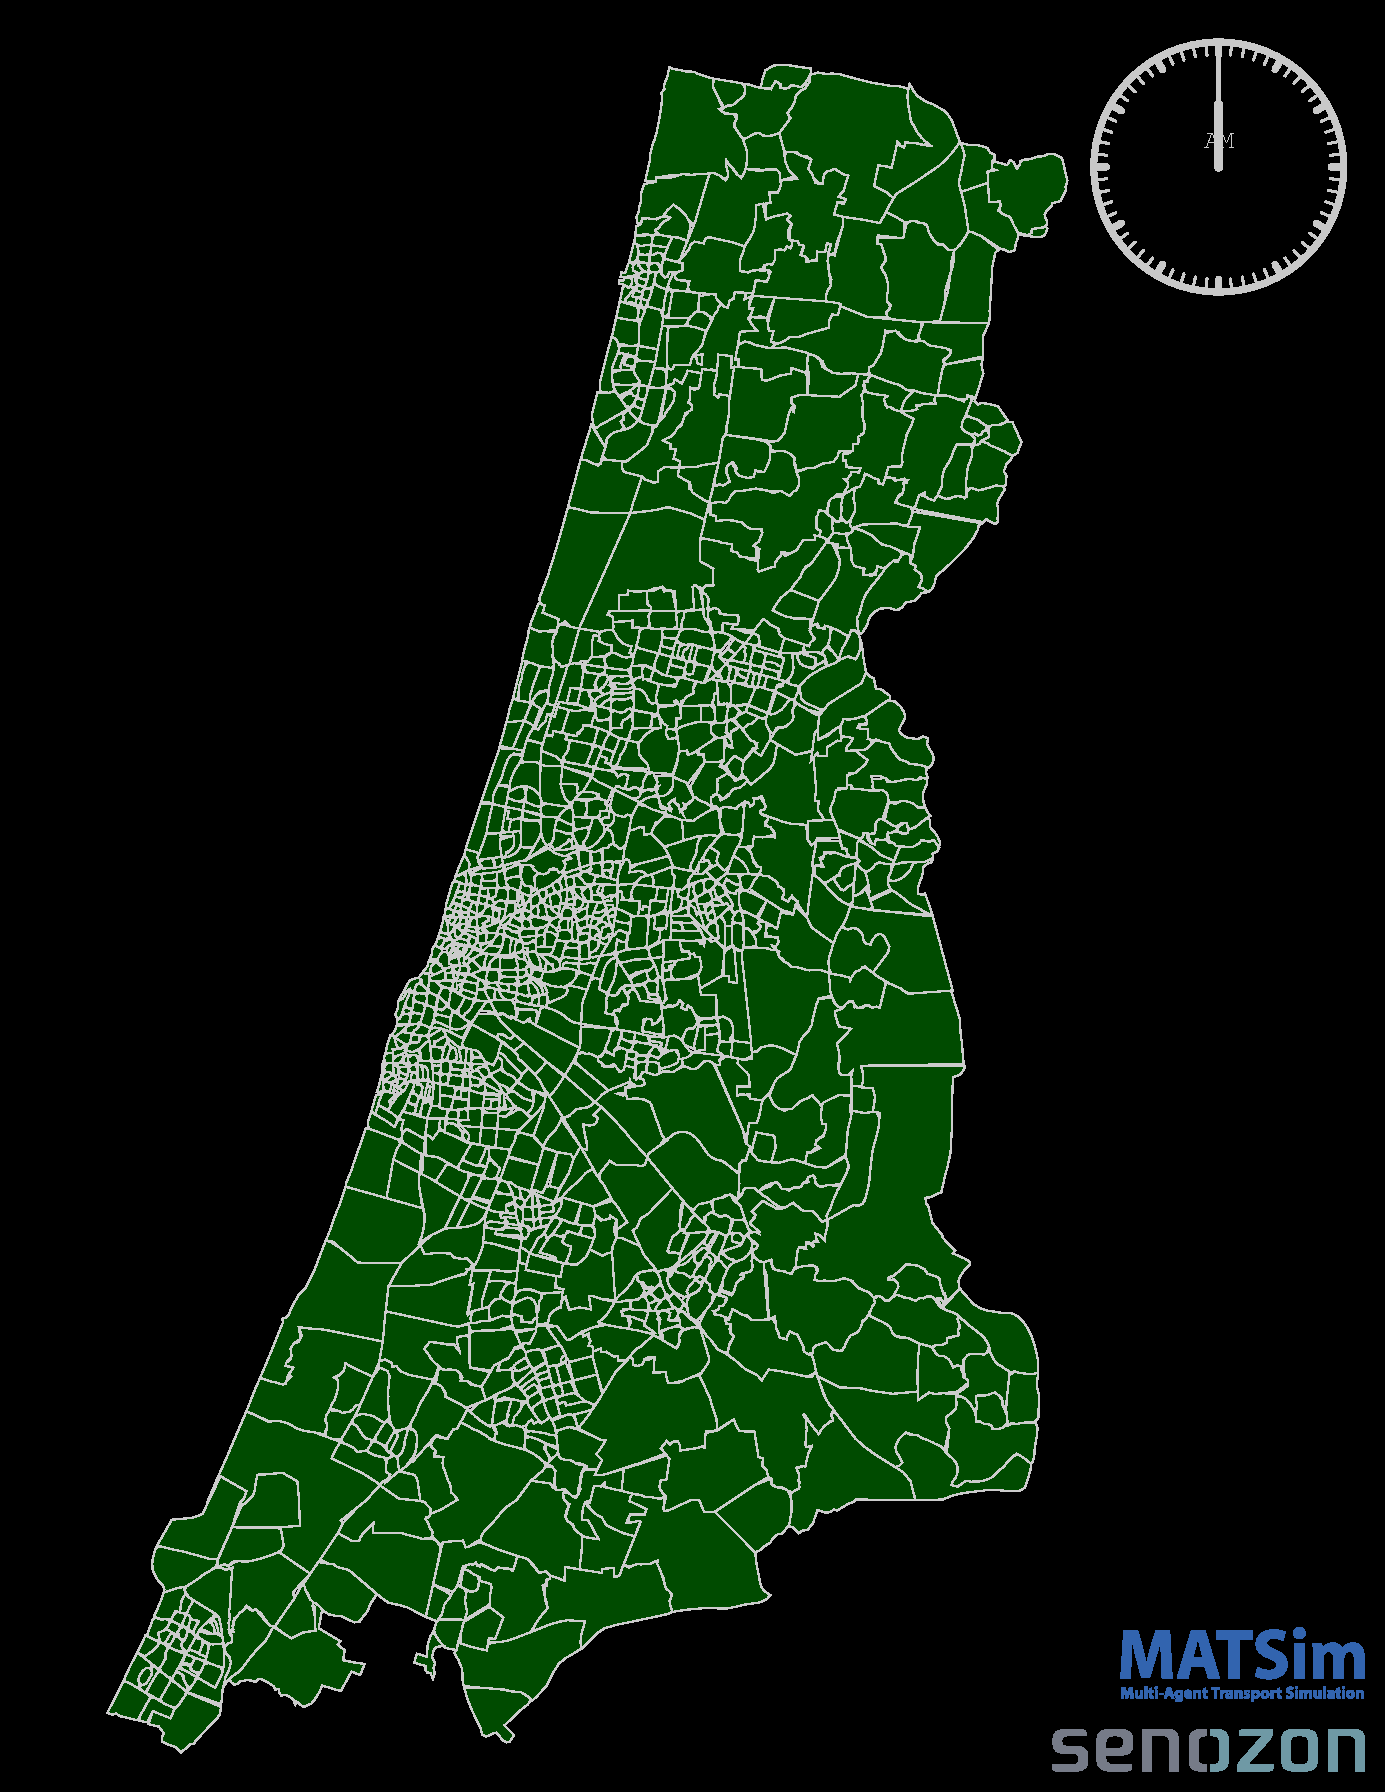
\includegraphics[width=0.49\textwidth,angle=0]{using/figures/TelAviv_TAZ}}%
  {\label{fig:TAZ}}%
  {}%
  \createsubfigure%
  {Network}%
	{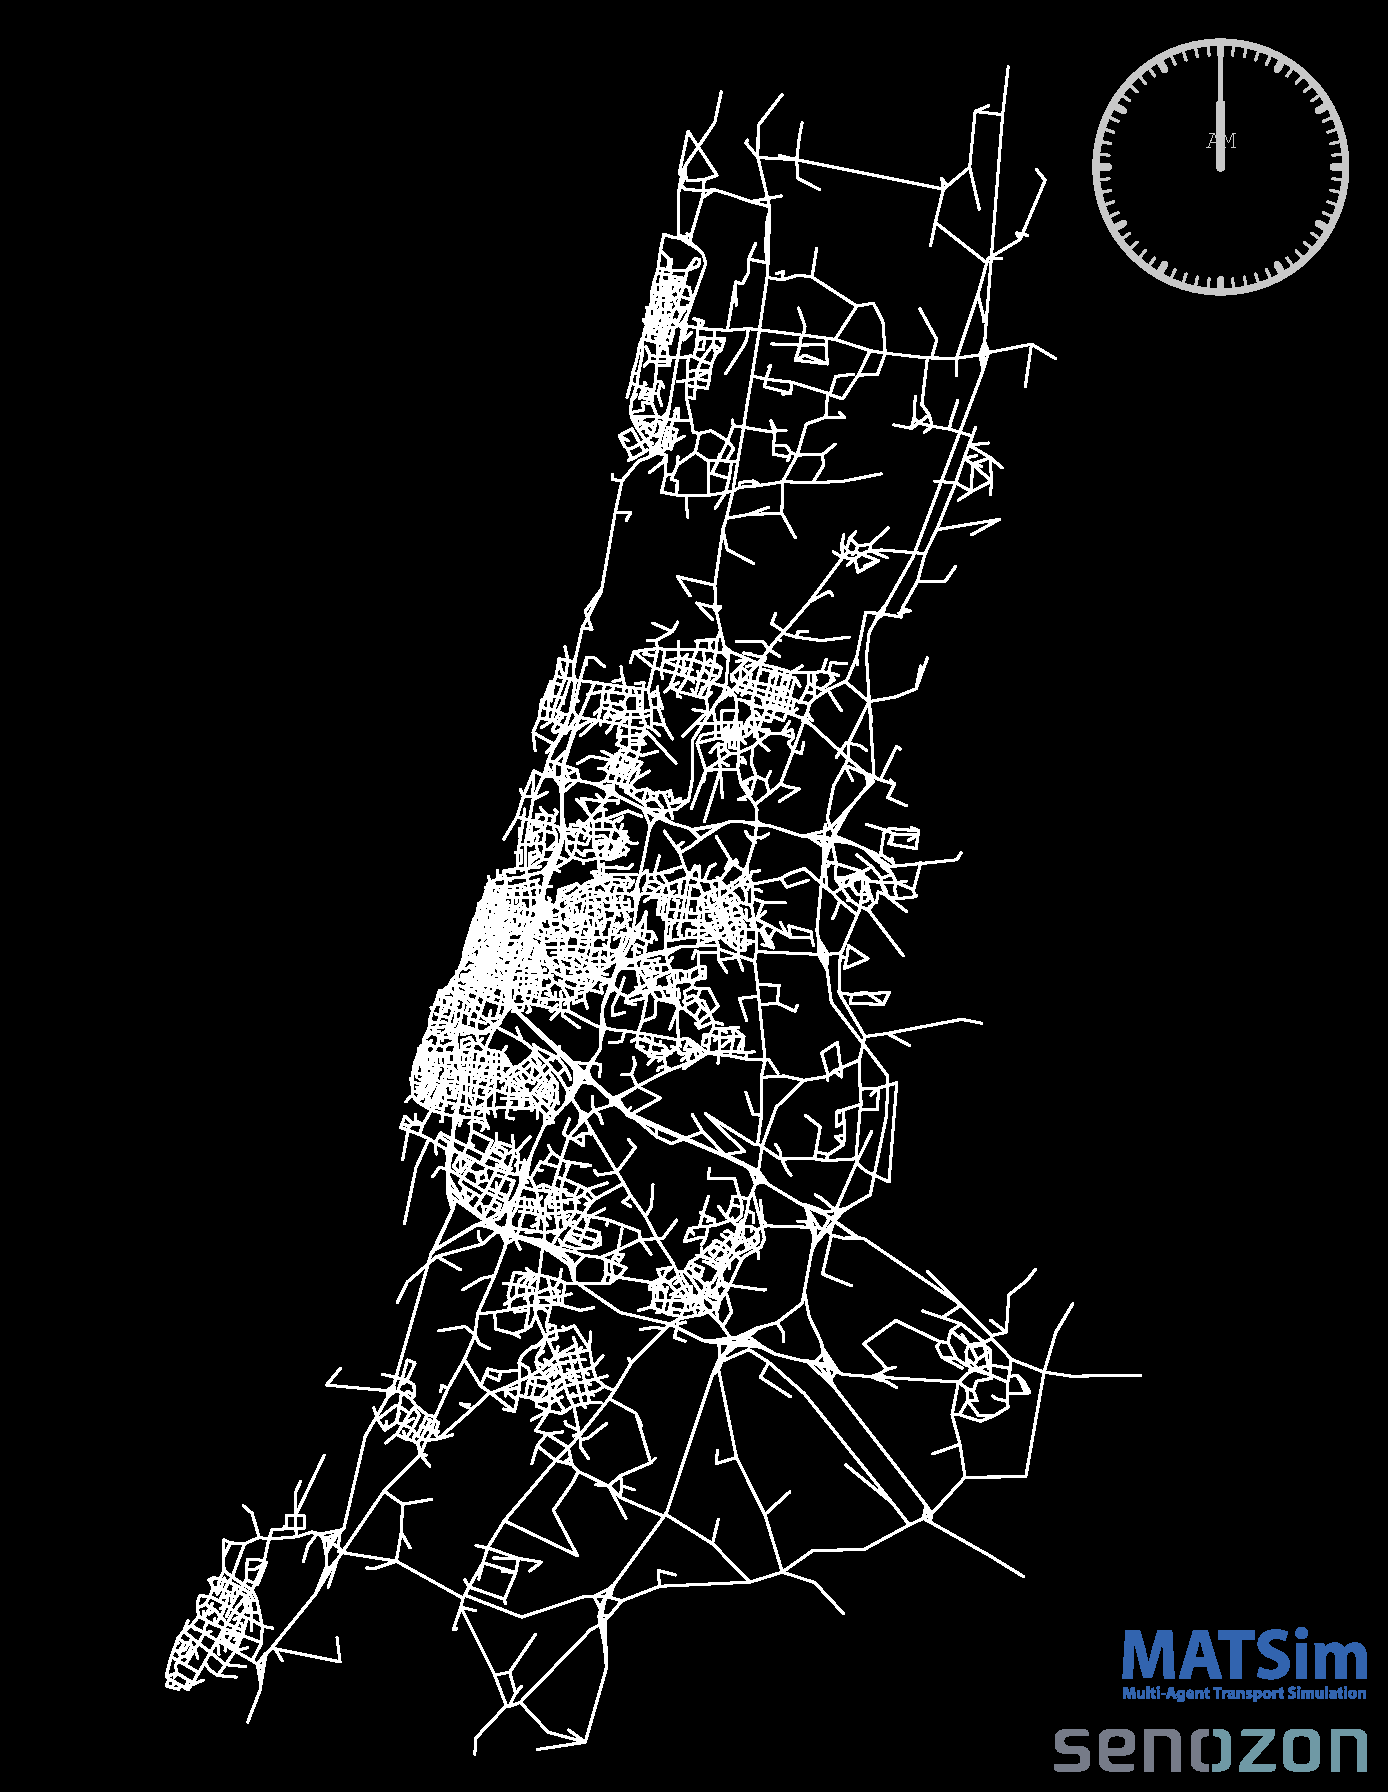
\includegraphics[width=0.49\textwidth,angle=0]{using/figures/TelAviv_RoadNetwork}}%
  {\label{fig:network}}%
  {}%
}%
{}

% ##################################################################################################################